\section{Prototype}
\label{sec:prototype}

%% \begin{figure}[t]
%%   \begin{center}
%%     \includegraphics[width=\columnwidth]{figures/process-model}
%%     \caption{\varan process model.}
%%     \label{fig:process_model}
%%   \end{center}
%% \end{figure}

\begin{figure}[t]
  \begin{center}
    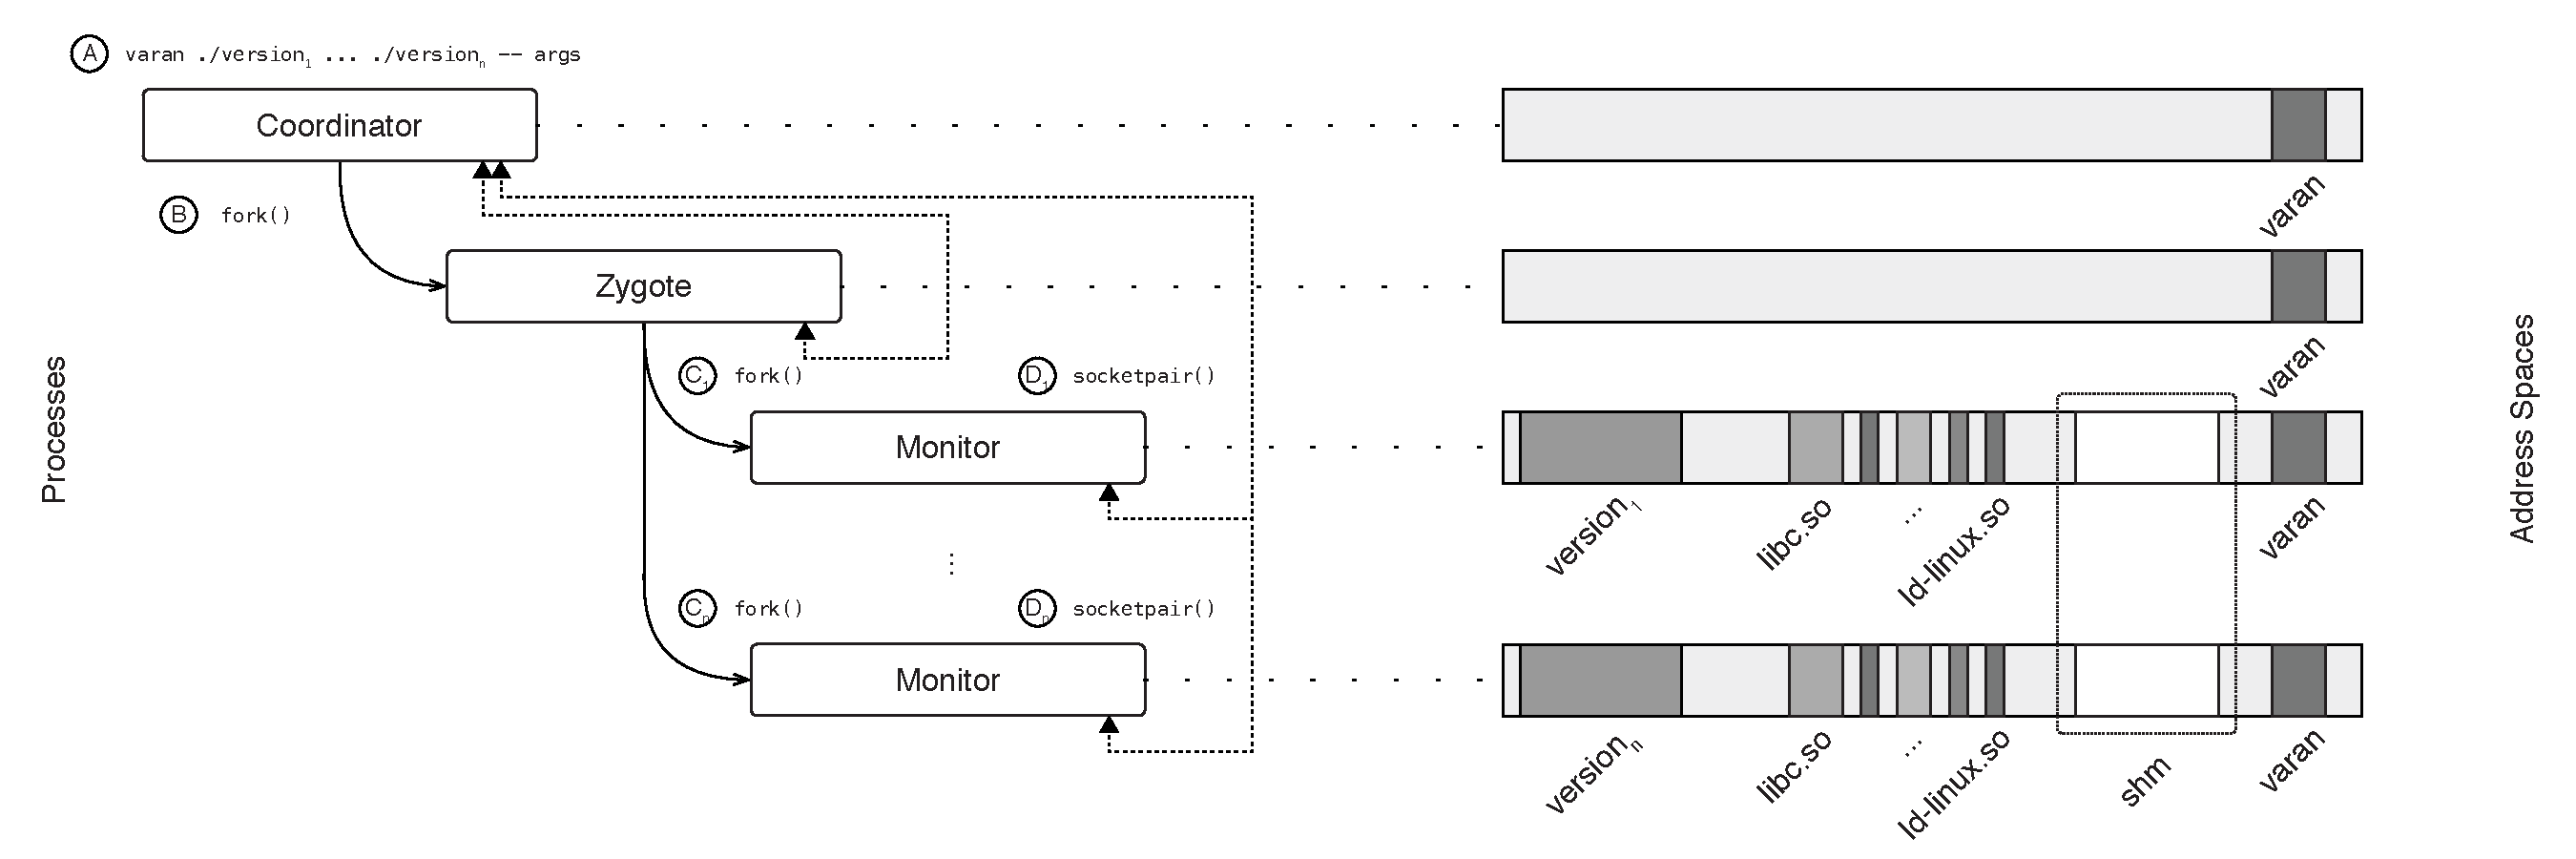
\includegraphics[width=\textwidth]{efficient-execution/figures/address-space}
    \caption{Setup of address spaces and communication channels.}
    \label{fig:setup}
  \end{center}
\end{figure}


We have implemented our approach in a prototype (to which we will also
refer as \varan), targeted at multi-core processors running x86-64 Linux.
\varan works on off-the-shelf binaries (both stripped and unstripped)
and supports single- as well as multi-threaded applications.

When it starts, \varan first sets up the address spaces of all program
versions and establishes the needed communication channels
(\S\ref{sec:setup}).  It then performs selective binary rewriting to
replace all system calls with  jump instructions
(\S\ref{sec:rewriting}).  After these initial stages, the event
streamer component of \varan ensures the coordination of the leader and
its followers (\S\ref{sec:streaming}).


\subsection{Setup of address spaces and communication channels}
\label{sec:setup}

The main steps involved in the setup of version address spaces and the
needed communication channels are shown in Figure~\ref{fig:setup}.  To
run multiple versions in parallel, the user launches \varan's
\emph{coordinator} providing the paths to all versions, together with
any command line arguments required to start them (Step \circl{A} in
Figure~\ref{fig:setup}).

% \begin{lstlisting}[language=bash,numbers=none]
% varan -p /path/to/executable1 
%         -p /path/to/executable2 -- args
% \end{lstlisting}

%The coordinator is linked with the \varan library (\varanlib, stored in
%\lstinline`libvaran.so`), which will be also injected inside each version.
%\varanlib is built as a statically-linked, position-independent library,
%to make sure it does not stand in the way of any segments which have
%to be loaded by the application at fixed addresses.

The \emph{coordinator} first creates the shared memory segment
used for communication among versions, and then spawns the
\textit{zygote} process (\circl{B}), which is responsible for starting
the individual versions. The coordinator communicates with the zygote
via a UNIX domain socket. For each version $i$ that needs to be spawned,
the coordinator sends a fork request to the zygote over this socket
pair, which includes the path to that version executable, the command
line arguments, and the end-point of a socket pair which will be used
for the subsequent communication between the coordinator and that
version (\circl{C$_i$}).
%
After receiving this request, the zygote spawns a new process, which
first finalises the communication with the coordinator
(\circl{D$_i$}).  The coordinator then sends the shared memory
segment descriptor to this process, which maps it inside its address
space.

%% returns a process identifier to the coordinator.  The coordinator then
%% sends the rank and shared memory segment descriptor to the version.

In the final step, the new process starts executing inside the monitor
code, which loads the specified ELF executable and sets up the initial
address space as described in the ELF headers. If the program requires
a dynamic linker, \varan loads the linker image specified in the
header as well.
%% Afterwards, \varan attaches the shared memory segment and initialises
%% the system call table based on the rank and arguments provided by
%% the coordinator.
The text segments of both the application and the dynamic linker are
then processed by the binary rewriter (\S\ref{sec:rewriting}). Finally,
\varan jumps to the application entry point as specified in the ELF header,
starting the execution of the application version.

The right-hand side of Figure~\ref{fig:setup} shows the address spaces
of the coordinator, zygote, and program versions.  When run with
\varan, program versions have two new segments mapped into their
address spaces: the shared memory segment used for communication among
versions (``shm'') and the \varan statically-linked library
(``varan'').  Note that \varan does not prevent address-space layout
randomisation schemes to be used by the operating system, because the
\varan library is compiled as PIC.

%% \varan is operates at the thin boundary between the operating system and
%% the user-space application---\ie below the C library and the dynamic
%% linker---and lives inside the address space of the host application;
%% however, the application itself is unaware of its existence.

% The rest of this section provides some extra details regarding the
% role and implementation of the coordinator, monitor and zygote.

\subsubsection{Coordinator}

To set up the address spaces of the versions, the coordinator acts as a
specialized preloader, inspired by
\emph{rtldi}.\footnote{\url{http://www.bitwagon.com/rtldi/rtldi.html}} However,
the coordinator does not attempt to replace the existing dynamic linker, which
would be unnecessarily complex and may affect compatibility with existing
applications. Instead, it simply intercepts the system calls performed by the
linker to enable the binary rewriter (\S\ref{sec:rewriting}) to rewrite the
code of dynamically-linked shared libraries.

One important advantage of our interception mechanism is that we do not make
use of \ptrace to intercept calls to the dynamic linker---instead, the binary
rewriter is used to rewrite all the system calls done by the linker with jumps
into the coordinator code.  As a result, \varan can be used in combination with
existing \lstinline`ptrace`-based tools such as \gdb or \textit{strace}, which
greatly simplifies debugging.

This architecture has several advantages over other commonly approaches. \varan
does not require the use of dynamic linker, as required by
\lstinline`LD\_PRELOAD`, and supports even statically linked applications.
This also has an advantage of supporting arbitrary dynamic linkers, not just
the one provided by \gnu C library, albeit it is going to be the most common
target.

\subsubsection{Zygote}

The role of the zygote is to spawn new processes on request from the
coordinator.  Zygote processes are already used in systems such as
\textit{Android} and \textit{Chrome}~\cite{linuxzygote}---in this paper, we use
the term to refer to the architectural pattern rather than a particular
implementation, as \varan provides its own clean-slate implementation.  While
it would be technically possible for the coordinator to create the processes in
which versions run, this would bring some complications regarding the
communication channels: for example, the second version spawned would inherit
the communication channel between the first version and the coordinator, which
would be undesirable.

\subsubsection{Monitor}

The monitor code is built as a statically-linked, position-independent library,
to make sure it does not stand in the way of any segments which have to be
loaded by the application at fixed addresses.  To ensure that the code can be
compiled like this, we must avoid using any global state (\ie any data that
would be placed in the ELF \lstinline`.data` section). One consequence is that
\varan cannot use any of the existing C libraries such as \textit{GNU C
Library}, as these are not typically built to support this requirement.
Instead, \varan provides its own implementation of the necessary C library
functions based on the \textit{Bionic C
library}.\footnote{\url{https://android.googlesource.com/platform/bionic}} To
support the use of Linux system calls, \varan uses a modified version of the
\lstinline`linux_syscall_support.h`
header.\footnote{\url{https://code.google.com/p/linux-syscall-support/}}

%% \varanlib provides its own entry point (\ie the \lstinline`\_start` function),
%% which is the starting point for \varan's execution. After start, it first
%% processes the arguments passed on stack by the Linux kernel, including
%% program arguments, environment variables and most importantly the
%% auxiliary data. Then, it loads the specified ELF executable into the
%% address space. Since \varan operates as a pre-loader, it is responsible
%% for setting up the initial address space layout as described by the
%% program header. If the program being executed requires dynamic linker,
%% \varan loads the linker image specified in the program header as
%% well. The text segments of both the application and the dynamic linker
%% are then processed by the binary rewriter (\S\ref{sec:rewriting}).


%% After start, \varan sets up the communication subsystem (\ie the shared
%% memory allocator, the ring buffer) and then forks the Zygote
%% process. The Zygote closes all open descriptors except for the socket
%% used as a communication channel with the coordinator and enters the
%% dispatch loop to wait for incoming requests. On fork request, the
%% Zygote receives command line arguments (\ie \lstinline`argv`) and a set of
%% file descriptors which will be available to the new process; then
%% forks itself and resumes to dispatch loop. The other type of requests
%% that Zygote supports are querying for process status (\ie equivalent
%% of \lstinline`waitpid`) and process termination (\ie \lstinline`SIGKILL`).

%% \begin{structure}
%% \item Establishing the initial memory layout as specified by the ELF
%% binary
%% \item Loading the dynamic loader (if specified by the ELF header)
%% \item Jumping to the application (or dynamic loader) entry point
%% \end{structure}


\subsection{Binary Rewriting}
\label{sec:rewriting}

%% \begin{structure}
%% \item Scanning each text segment in the program address space
%% \item Rewriting every syscall with jump instruction where possible,
%% otherwise using interrupt
%% \item Using table of system call handlers to interpose on selected
%% system calls
%% \end{structure}

To intercept system calls, \varan uses selective binary
rewriting~\cite{bird}. Unlike traditional dynamic binary rewriting
implemented by tools like DynamoRIO~\cite{dynamorio02} or
Pin~\cite{pin05}, where the entire process image is being rewritten,
often introducing a significant performance overhead, \varan only
replaces the instructions for performing system calls (\ie
\lstinline[language={[x64]Assembler}]`int $0x80` on x86 and
\lstinline[language={[x64]Assembler}]`syscall` on x86-64).
%% This approach has been originally implemented in
%% \emph{BIRD}~\cite{bird} for the Windows/x86 platform and later in
%% \emph{seccompsandbox}\footnote{\url{https://code.google.com/p/seccompsandbox/}}
%% for Linux. 
%Our implementation extends the \emph{seccompsandbox}\footnote{\url{https://code.google.com/p/seccompsandbox/}} framework for Linux.

The rewriting itself is done when a segment is mapped into memory with
executable permissions, or an existing memory segment is marked as
executable.  
%(\ie \lstinline`mmap` system calls with executable flag, typically
%performed by the dynamic linker).
During rewriting, \varan scans the segment searching for system call
instructions using a simple x86 disassembler.  Every system call found
is rewritten with a jump to an internal system call entry point. This
process is complicated by the fact that while a system call
instruction is only one byte long, a jump instruction requires five
bytes.  Therefore, in order to rewrite the system call with a jump, we
also need to relocate some of the instructions surrounding the system
call---\ie perform binary detouring via trampolines~\cite{detours}.
On the rare occasions when this is not possible (\eg because the
surrounding instructions are potential branch targets), we replace the
system call with an interrupt (\ie \lstinline`INT 0x0`) which has the
same size as system call instruction (\ie \lstinline`INT 0x80`) on
x86-32 and \lstinline`SYSCALL` on x86-64).  This interrupt is handled by
\varan through a signal handler installed during initialisation, which
redirects the control flow to the system call entry point as for other
system calls.

The system call entry point first saves all registers, and then
consults an internal system call table to check whether there is a
handler installed for that particular system call; if so, it calls
that handler, otherwise it invokes the default handler.  After
processing the system call, the entry point handler restores all
registers and returns to the original caller (using
\lstinline`sigreturn` in the case of system calls intercepted via an
interrupt). The system call entry point also implements support for
restarting system calls (\ie signaled by the \lstinline`-ERESTARTSYS`
error code). This is used in certain scenarios supported by \varan
including transparent failover (\S\ref{sec:applications}).

The internal system call table can be easily changed to accommodate
various application scenarios.  In particular, the only difference
between the leader and the followers is the system call table. For
example, the \lstinline`write` system call would be redirected in the leader
to a function that performs the call and records its result in the
shared ring buffer, while in the followers it would be redirected to a
function that reads the results from the shared buffer without making
the call.
%% \varan allows both the system call table and the default system call
%% handler to be provided by the embedder of \varan \todo{Where shall we
%%   described the possibility of \varan embedding, \ie building tools on
%%   top of \varan?}. This makes it easy to customize \varan behavior for
%% different use cases (\S\ref{sec:failover}). For our prototype, we have
%% provide three different system call tables (\ie record, replay and
%% passthrough). 
\varan  also provides a Python script which can produce new tables
and their implementations using templates.
%% ; in fact, the passthrough table was implemented using this
%% generator. We have also used the generator throughout the \varan
%% development for testing and debugging purposes.

Finally, note that in order to prevent potential attackers to easily inject
system calls into the program, the binary rewriter follows a
W$\mathbin{\oplus}$X discipline throughout execution, making sure that
segments are not marked as both writable and executable at the same
time.


\subsubsection{Virtual System Calls}
\label{sec:vsyscall}

Certain Linux system calls are accelerated through the \emph{vsyscall}
page and the \emph{vDSO} segment. These are mapped into the address
space of each Linux process, and contain system call
implementations. These \textit{virtual system calls} do not incur the
context switch overhead between kernel and user space associated with
standard system calls.

The \emph{vsyscall} page was introduced first, but is being deprecated in favor
of the \emph{vDSO} segment.\footnote{We are referring to x86-64 version, on x86
systems the vDSO segment contains a function used to determine the preferred
method of making a system call} The main reason for this development is that
the \emph{vsyscall} page is mapped to a fixed address, making it susceptible to
return-oriented programming attacks~\cite{ROP:tissec12}. To address this issue,
the vDSO segment is mapped to a random address. Since the segment is
dynamically allocated, it can also support an arbitrary number of virtual
system calls (currently \lstinline`clock_gettime`, \lstinline`getcpu`,
\lstinline`gettimeofday` and \lstinline`time`).

On x86-64 system, Linux would map a vDSO segment into each process' address
space. This segment contains a fully formed ELF image with function symbols
prefixed with \lstinline`__vdso_`, one for each virtual system call.
Applications can then call these functions and avoid performing a full context
switch into kernel associated with a regular systems call. However, in practice
applications are more likely to use a wrapper provided by their C library such
as \gnu C library, which checks whether the vDSO page is available and if so
uses the virtual system call, or alternatively falls back to the regular system
call implementation.

Virtual system calls represents one of the major limitations of
\lstinline`ptrace`-based monitors. Since these system calls are entirely
implemented in user space, they cannot be intercepted via \ptrace.
This is an important limitation: as these system calls provide access
to timing information, they are often used as a source of
non-determinism (\eg for random number generators) and their handling
is critical for any NVX system. %Despite this, previous systems either
%omit discussion on virtual system call handling~\cite{mx,orchestra11}
%or explicitly mention their inability to handle them~\cite{tachyon12}.

To our knowledge, \varan is the first NVX system which handles virtual system
calls, using binary rewriting.  Previous systems either omit discussion on
virtual system call handling~\cite{orchestra11} or explicitly mention their
inability to handle them~\cite{tachyon12}.
%In \varan, binary rewriting is also used to intercept virtual system
%calls.
Handling calls made via the \textit{vsyscall} page is easier because
the function symbols are always mapped to the same address.  
%% We can therefore easily identify calls to these functions while
%% scanning the text segment and rewrite them to calls into our system
%% call table.
To handle \textit{vDSO} calls, we first need to determine the base
address of the \textit{vDSO} segment; this address is passed by the
kernel in the ELF auxiliary vector via the \lstinline`AT_SYSINFO_EHDR`
flag.\footnote{\url{https://www.gnu.org/software/libc/manual/html_node/Auxiliary-Vector.html}}
Second, we need to examine the ELF headers of the \textit{vDSO}
segment to find all symbols.  Identifying calls to these symbols is
more complicated than in the \textit{vsyscall} case because these
symbols are allocated at arbitrary addresses.  Instead, we replace the
entry point of each function with a jump to dynamically generated code
which sets up the stack and then issues a call to the \varan system
call entry point as in the case of regular system calls. Furthermore, we
provide a trampoline, which allows the invocation of the original
function, by moving the first few instructions of each function to a
new place, followed by a jump to the original code. This allows \varan
to take advantage of the virtual system call mechanism to further
improve performance.

%% Finally, we note that this function interception mechanism is not
%% specific to system calls and can be used to intercept arbitrary
%% functions in the target application if needed, similarly to
%% Detours~\cite{detours}.



\subsection{Event Streaming}
\label{sec:streaming}

%% \begin{structure}
%% \item Externally observable behavior triggers events (\eg system calls,
%% signals), these events are being recorded and replayed by individual
%% versions
%% \item The concept of event-streaming; all versions share a common event
%% stream (\ie log) of fixed size
%% \item One version is always elected as a leader adding new events to the
%% stream, the other versions are followers replaying the events from the
%% stream
%% \item When the leader crashes, followers elect a new leader
%% \end{structure}

As we discussed briefly in Section~\ref{sec:overview} and illustrated
graphically in Figure~\ref{fig:architecture}, the leader records all
external events into a shared ring buffer, while the followers replay
them to mimic the leader's behavior. The leader is the only version
interacting with the environment, \ie executing the system calls, with
the exception of system calls which are local to the process (\eg
\lstinline`mmap`). % or \lstinline`sigaction`).

As in any NVX system operating at the level of system calls, \varan
has to be aware of the system call semantics, in order to transfer the
arguments and results of each system call.  \varan currently
implements \syscallsHandlers system calls, which were all the system
calls encountered across our benchmarks.\footnote{We configured \varan
  to emit an error message when an unhandled system call is
  encountered, and have implemented system call handlers on demand.}

%% All application instances running in parallel under \varan are assigned
%% ranks, similarly to OpenMPI~\cite{OpenMPI}. The instance\footnote{We
%%   refer to the instances rather than a process as application may have
%%   multiple threads/subprocesses} with rank 0 is denoted as
%% \emph{leader} while all other instances are denoted as
%% \emph{followers}. 


%% When followers would execute a system call under normal execution, now
%% they simply return a value from the event stream (\ie the return value
%% of the system call executed by the leader).

% \varan recognizes several different types of events:
% \begin{inparaenum}[(i)]
% \item \emph{syscall} for the system call entry,
% \item \emph{sysret} for the system call exit,
% \item \emph{signal} for an interceptable signal,
% \item \emph{exit} for the process exit.
% \end{inparaenum}
% Furthermore, it is possible to add other types of events if necessary.

%% Each event has a fixed size of 64 bytes where first byte is
%% used as an event type.  The size has been deliberately chosen to be
%% fit into a single cache line on modern x86 CPU (see \S\ref{sec:ipc}
%% for more details).

%% \subsection{Interprocess Communication}
%% \label{sec:ipc}

%% \begin{structure}
%% \item Sending events from one process to other without the use of system
%% calls to avoid the additional overhead
%% \item Shared memory queues for process to process communication
%% \item Custom shared memory allocator with reference counting
%% \end{structure}

%% Since one of our primary goals for \varan was to minimize the performance
%% overhead, to avoid additional system calls being made during system
%% call handling (\S\ref{sec:overview}), we have designed an interprocess
%% communication mechanism which does not use system calls (\eg
%% socket-based communication primitives).

\subsubsection{Shared ring buffer}
\label{sec:ring}

For fast communication, the leader and its followers share a common
ring buffer of fixed size, which is held entirely in memory.  Our
initial solution used a separate shared queue for each
process~\cite{fastforward,mcringbuffer}, with the
%% Shared memory queues are often used for fast core-to-core
%% communication in high-performance applications.
coordinator acting as an event pump---reading events from the leader's
queue and dispatching them into followers' queues.  This approach
worked well for a low system call rate, but at higher rates the event
pump quickly became a bottleneck.  
% Furthermore, although we used a
% state-of-the-art shared queue implementation~\cite{bqueue}, we still
% experienced a large performance overhead for system call
% interception---over $20\times$ for a worst-case microbenchmark,
% compared to $4\times$ in the final implementation.

As a result, we have instead opted for a design based on the Disruptor
pattern~\cite{disruptor}, which uses a shared ring buffer allowing concurrent
access by multiple producers and consumers, eliminating the need to dispatch
events among queues, and thus improving both performance and memory
consumption.  Our implementation uses C11 atomics, 
%introduced in C11 and now supported by both GCC and Clang, 
in combination with cache aligning to
achieve maximum performance with minimal use of locking (locks are used only
during memory allocation and deallocation).

%The ring buffer is used to stream events between processes.  
The size of the ring \varan uses is configurable and has a default
value of 256 events.  Each event has a fixed size of 64 bytes; the
size has been deliberately chosen to fit into a single cache line on
modern x86 CPUs.  This is sufficient for sending signals and system
calls for which all arguments are passed by value (on x86-64, a system
call can have up to six arguments of eight bytes, to fit into general
purpose registers).  However, for system call arguments passed by
reference, the payload might have variable size and can be potentially
larger than the event itself.  In this case, we use events only to
transfer shared pointers, which identify memory shared across
versions.

The use of a shared memory buffer may result in a waste of system
resources when the leader process performs a system call which blocks
for a long period of time, as the followers use busy waiting to check
for new events. To address this problem, we have introduced the
concept of a \emph{waitlock}. Whenever a follower makes a blocking
system call, it acquires the waitlock. If there is no event available,
the thread will block until the leader wakes up and notifies it. The
waitlocks are efficiently implemented using a combination of C11
atomics and futexes~\cite{futex}.

\subsubsection{Transferring file descriptors and leader replacement}
\label{sec:leader-repl}

Apart from the ring buffer, each version has a \textit{data channel},
implemented using UNIX domain sockets.
% Together, the ring buffer and data channel form an \emph{event
% stream} which is a primary communication mechanism for exchanging
% events among instances.
The data channel is used to send information which cannot be
transferred via shared memory, in particular open file descriptors.
Whenever the leader obtains a new file descriptor (\eg by opening a
file), it sends this descriptor to all followers, effectively
duplicating the descriptor into their processes. This is a crucial
mechanism which enables the leader to be replaced transparently when
it crashes. When the leader crashes, the follower that is elected as
the new leader can simply continue executing using existing
descriptors (\eg responding to requests coming over the network)
without any disruption of service.

% Currently, UNIX domain sockets do not support broadcast, so the leader
% communicates with the followers via the coordinator, which then sends
% the descriptor separately to all followers.  However, there are
% proposals to add broadcast support for UNIX domain
% sockets,\footnote{\url{https://lkml.org/lkml/2012/2/20/208}} which would
% simplify the design of our prototype and further improve performance.


\subsubsection{Multi-process and multi-threaded applications}
\label{sec:threading}
\label{sec:ipc}

Handling processes and threads is crucial in supporting many modern
applications.  
%The discussion below refers to processes, but threads are handled in a
%similar way.
In our design, we have opted to have separate ring buffers for each
tuple of processes or threads in the system: for instance, when a
process forks, the parent processes in the leader and all followers
form one tuple, and the child processes another, with a process in
each tuple acting as the leader.  More exactly, when a new process is
forked, a new socket pair is established between the process and the
coordinator and a new ring buffer is allocated.  The leader then
continues execution, but the coordinator waits until all followers
fork a new process, establishing appropriate socket pairs for
communication, and setting the child processes to read events from the
newly-allocated ring buffer.

To alleviate non-determinism issues due to scheduling, \varan enforces
system call ordering across all tuples using Lamport's
\emph{happens-before} relation~\cite{lamport78}. Currently, this is
only implemented for multi-threaded applications, which make intensive
use of synchronisation primitives, but the same solution could be
employed for multi-process applications too.

\begin{figure}[t]
  \begin{center}
    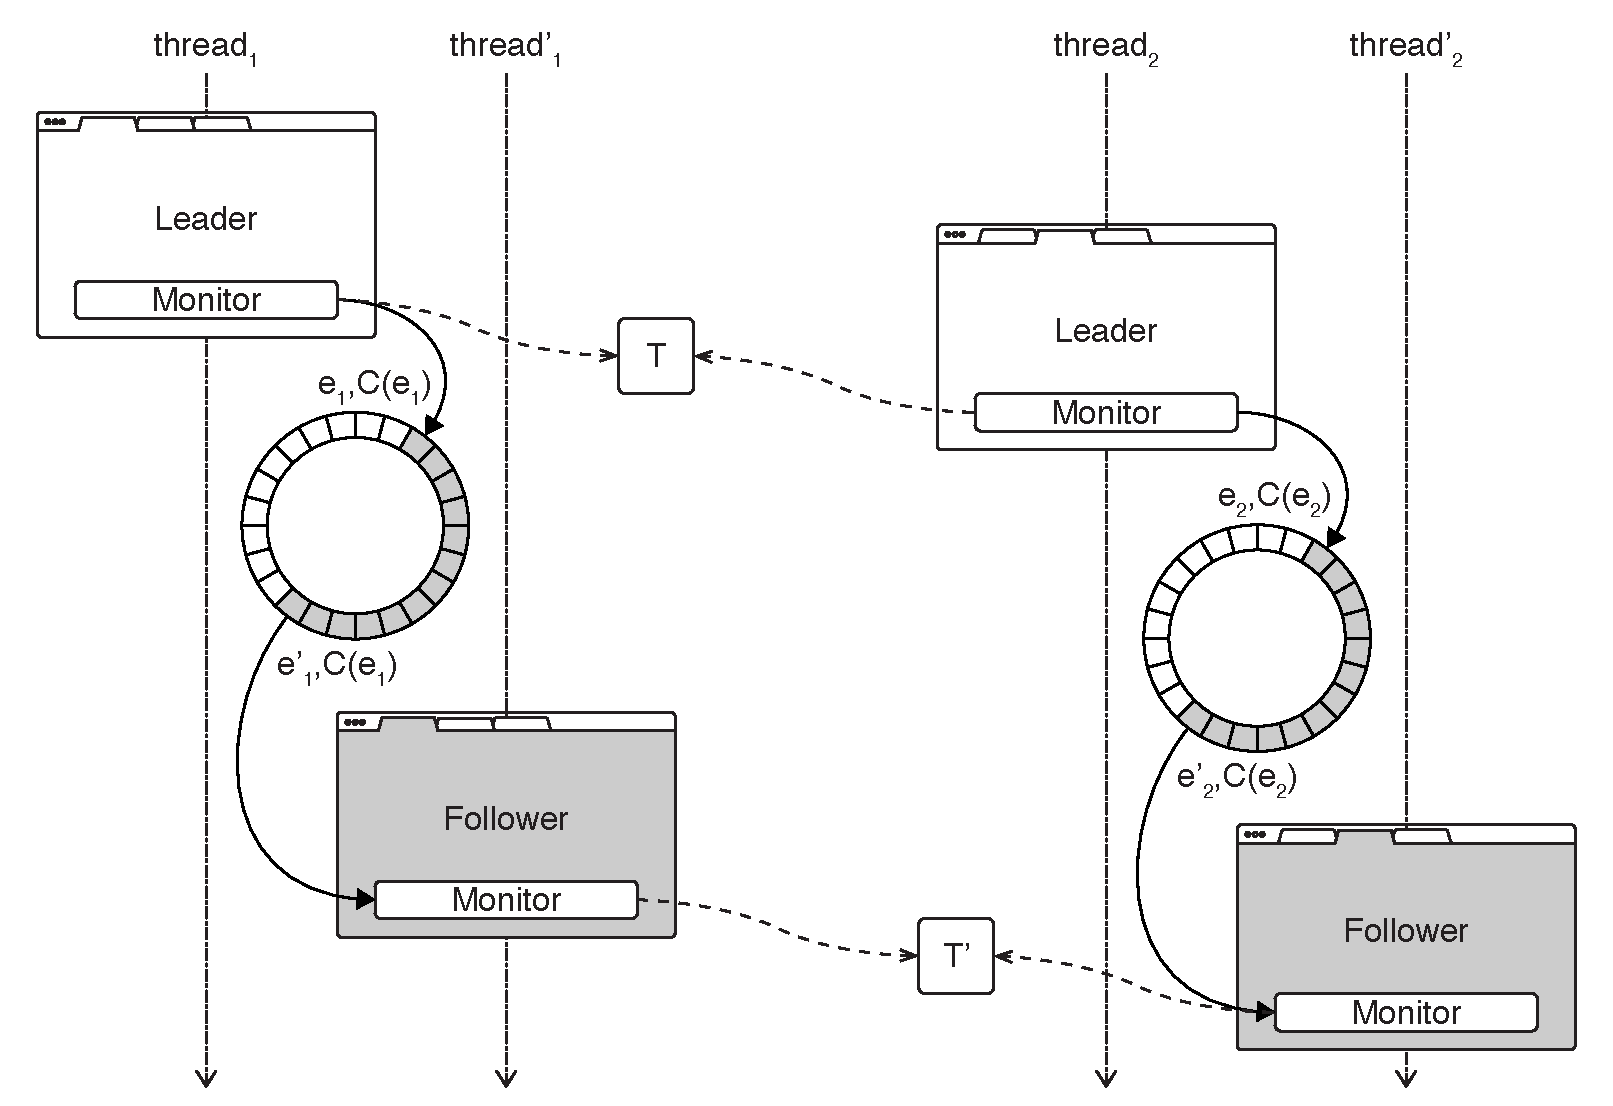
\includegraphics[width=0.75\textwidth]{efficient-execution/figures/multithreading}
    \caption{Event delivery in a multi-threaded NVX program, with
      the ordering of events enforced using logical clocks.}
    \label{fig:multithreaded}
  \end{center}
\end{figure}

Each variant has an internal Lamport clock, shared by all threads, and
each event $e_i$ sent through the ring buffer is annotated with a
timestamp $C(e_i)$.  Then, when replaying events from the buffer, each
thread checks the timestamp of every new event and only receives the
event if it does not violate the happens-before relation. This
scenario is depicted in Figure~\ref{fig:multithreaded}. If $e_1\to
e_2$ ($e_1$ happens before $e_2$), then $C(e_1)<C(e_2)$ and \varan
enforces $e'_1\to e'_2$. Without the ordering, there could be a
situation where $e_1\to e_2$, but $e'_1\not\to e'_2$, which could lead
to a divergence. A similar approach has been proposed in the past for
record-replay in shared-memory systems~\cite{levrouw94}.

To implement the internal clocks shared by the threads of a variant
($T$ and $T'$ in Figure~\ref{fig:multithreaded}),
we use an atomic counter allocated in the shared memory space and
updated using C11 atomics for efficiency.  When the leader thread
writes a new event into the ring buffer, it increments its variant's
clock value and attaches it to the event.  When a follower thread
reads an event from the ring buffer, it compares its variant's clock
value with the event's timestamp.  If they are equal, the thread
increments its variant's clock value and processes the event,
otherwise it continues waiting. Our current implementation uses busy
waiting, as the wait times are expected to be small.  However, shall
this become a problem in the future, it is possible to use blocking
wait instead (\eg a futex).

% Since Disruptor (\S\ref{sec:ring})
% allows concurrent writes by multiple producers without the need for
% expensive synchronisation, the use of a single shared buffer does not
% create a performance bottleneck. %hinder the application performance.

Our solution resembles existing deterministic multi-threading (DMT)
mechanisms~\cite{coredet:asplos10,dthreads:sosp11}. The guarantees
provided by \varan are weaker than those typically provided by these
systems as we do not enforce ordering across atomics-based
synchronisation primitives. We have not detected any system call
divergences caused by related data races in our benchmarks, which
include multi-threaded applications (\eg \redis), similar to the
experience reported for prior NVX systems. However, shall this become
a problem, we could address it by employing a stronger form of
determinism similar to existing DMT systems.

%
% However, this weaker form of determinism
% does not typically pose a problem for real-world applications as long
% as they are properly synchronised.  Note that data races resulting
% from missing or incorrect synchronisation can cause followers to issue
% a different sequence of system calls from the leader.  If this
% happens, we could either try to apply one of the rewriting rules
% (\S\ref{sec:patternmatching}), or terminate the follower.
%

%% Each instance also has a dedicated \emph{service channel}, similarly
%% to the data channel implemented using UNIX domain sockets. The service
%% channel is used to transfer commands and service requests between
%% coordinator and the instance.

%% One such example are \lstinline`fork` and \lstinline`clone` system calls. The new
%% process spawned as a result of these system calls needs to have its
%% own data and service channel. The parent process is responsible for
%% creating these using a \lstinline`sockepair` system call. One end of each
%% pair is inherited by the new process while the other end is sent to
%% the coordinator where it is associated with the new process.

%Note that data races resulting from missing or incorrect
%synchronisation can cause followers to issue a different sequence of
%system calls from the leader.  If this happens, that follower would
%have to be terminated.  We first note that \varan has not detected any
%system call divergences caused by data races in our benchmarks (which
%include many popular applications such as \apache, \nginx, and \redis),
%so this might not be such an important aspect in practice.  Prior NVX
%systems do not address this problem either, likely due to a comparable
%experience.

%However, we envision two possible solutions.  The first one would be
%to use deterministic multi-threading (\eg
%Dthreads~\cite{dthreads:sosp11}).  The second solution would be to
%allow developers to document any benign races as rewrite rules
%(cf. \S\ref{sec:patternmatching}).

\subsubsection{Memory allocation scheme}  

Efficient shared memory allocation plays an important role in a system
like \varan.  We use a custom shared memory pool allocator implementation.
%, similar to the one used by OpenMPI.\footnote{\url{http://www.open-mpi.org/}}
The allocator has the notion of buckets for different allocation sizes,
where each bucket holds a list of segments, and each segment is
divided into chunks of the same size; each bucket holds a free list of
chunks.  When there are no more unused chunks in a bucket, the
allocator requests a new segment from the memory pool, and divides it
into chunks which are then added to the free list. Each bucket also
has a lock associated with it which has to be held prior to an
allocation from that bucket. 
% While this design is relatively simple,
% it performed well in our benchmarks. We also experimented with
% more advanced designs (\eg using different allocation strategies for
% smaller and larger blocks), but the basic allocator always
% outperformed all other implementations.  

%% However, we believe it might still be possible to come with a more
%% specialized allocation strategy which would further improve the
%% performance of \varan, and this is something we would like to address in
%% our future work.

%% The critical part of many systems which use shared memory for
%% communication is deallocation. There are various solutions to this
%% problem. One possibility is to use some form of garbage collection,
%% such as reference counting. Unfortunately, this solution is not
%% applicable in our case since the leader is not aware of any of the
%% consumers processing its events making it difficult to consistently
%% manage the reference counts. The original Disruptor implementation,
%% which targets the Java runtime simply relied on the garbage collector
%% provided by the virtual machine. Unfortunately, this solution is not
%% applicable in our case either. Instead, we have extended the C-based
%% Disruptor implementation to notify a follower if it is the last one
%% that processes an event. \todo{how?}  If that is the case, the
%% follower is responsible for freeing the associated memory. This
%% solution does not add any overhead and does not require any
%% modifications to the allocator.

% This property allows us sharing memory between individual application
% instances without explicitly tracking which instance is responsible for
% deallocation, or using the back channel to notify instance that the block is
% available for deallocation as in the case of OpenMPI

\subsection{Rewrite rules for system call sequences}
%\subsubsection{System call filtering and rewriting}
\label{sec:patternmatching}

\varan uses Berkeley Packet Filters (BPF)~\cite{bpf} to implement the system call
rewrite rules introduced in Section~\ref{sec:rw}.  BPF is a machine
language for writing rules and an interpreter shipped with many UNIX
implementations, including Linux and BSD.  BPF filters have been
traditionally used to filter network packets, but recently also for
system call filtering as a part of seccomp ``mode 2'' (also known as
seccomp-bpf).

We have integrated a BPF interpreter in \varan to allow for system
call rewrite rules. Our implementation is based on the Linux kernel
code which was ported to user space and extended for NVX
execution. \varan provides BPF extensions on top of the instruction
set used by seccomp-bpf.\footnote{\url{https://www.kernel.org/doc/Documentation/networking/filter.txt}}
The \lstinline[language={[bpf]Assembler}]`event` extension allows
access to the event stream, which can be used to compare the system
calls executed across versions, as we will show in
Section~\ref{sec:mv-execution}.

%We have also made the offset, used to access the \lstinline`struct seccomp_data` content writable.

% This required adding a new return value
% \lstinline`SECCOMP_RET_REPLACE` where the bottom 16-bits of the return
% value specify the new system call number the original system call is
% going to be rewritten to.  Since these extensions does not add any new
% instructions or extend the semantics of the BPF language, the
% \lstinline`bpf_asm` tool can be used to compile the filters into a
% binary form. This can be then loaded into \varan on start through a
% command line option.


The use of BPF has a number of advantages.  First, it does not require
the user to modify and recompile the monitor on every rule
change. This is particularly important as rewrite rules can be
application specific. Second, the BPF machine language was designed to
be simple enough to prevent certain classes of errors---in particular,
all filters are statically verified when loaded to ensure termination.
% (\ie every filter has to end with a \lstinline`ret` instruction).



%We also argue that the choice of BPF as a language for stream rewriting rules
%makes it easier to adopt by administrators, the most likely users of \varan,
%compared to some other more esoteric languages such as Haskell~\cite{tachyon}.

%% \begin{lstlisting}{language=[bpf]Assembler,caption={Example of a BPF rewriting rule}}
%% ld [0]                /* offsetof(struct seccomp_data, nr) */
%% jne #1, good          /* __NR_write */
%% bad: ret #0           /* SECCOMP_RET_KILL */
%% ldi #18               /* __NR_pwrite */
%% add #0x00070000       /* 18 + 0x00070000 */
%% ret %a                /* SECCOMP_RET_REWRITE */
%% good: ret #0x7fff0000 /* SECCOMP_RET_ALLOW */
%% \end{lstlisting}
